% 
% Lecture Template for ME3023 -  Measurements in Mechanical Systems - Tennessee Technological University
%
% Spring 2020 - Summer 2020
% Tristan Hill, May 07, 2020 - June 12, 2020 - July 08, 2020
% Module X - Electrical Instruments
% Topic 2 - More Instruments
%


\documentclass[fleqn]{beamer} % for presentation (has nav buttons at bottom)

\usepackage{/home/thill/Documents/lectures/measurements_lectures/measurements_lectures}

\author{ME3023 - Measurements in Mechanical Systems} % original formatting from Mike Renfro, September 21, 2004

\newcommand{\MNUM}{5\hspace{2mm}} % Module number
\newcommand{\TNUM}{2\hspace{2mm}} % Topic number 
\newcommand{\moduletitle}{Electrical Instruments}
\newcommand{\topictitle}{More Analog Instruments} 

\newcommand{\sectiontitleI}{Safety and Electricity }
\newcommand{\sectiontitleII}{Using a Desktop Power Supply}
\newcommand{\sectiontitleIII}{Using a Function Generator}
\newcommand{\sectiontitleIV}{Using an Oscilloscope}


% custom box
\newsavebox{\mybox}

\title{Lecture Module - \moduletitle}

\date{Mechanical Engineering\vspc Tennessee Technological University}

\begin{document}
	
	\lstset{language=MATLAB,basicstyle=\ttfamily\small,showstringspaces=false}
	
	\frame{\titlepage \center\begin{framed}\Large \textbf{Topic \TNUM - \topictitle}\end{framed} \vspace{5mm}}
	
	
	% Section 0: Outline
	\frame{
		\large \textbf{Topic \TNUM - \topictitle} \vspace{3mm}\\
		
		\begin{itemize}
			
			\item \sectiontitleI    \vspc % Section I
			\item \sectiontitleII 	\vspc % Section II
			\item \sectiontitleIII 	\vspc %Section III
			\item \sectiontitleIV 	\vspc %Section IV
			
		\end{itemize}
		
	}



\section{\sectiontitleI}

% Section I - Frame I:
\frame{  \small
\frametitle{\sectiontitleI}



Please read the {\bf In-Lab Safety and Good Practices} document \textbf{or} \vspace{3mm}\\
the {\bf Remote-Lab Safety and Good Practices} document. \vspace{10mm}\\

Also, stay tuned for information about your lab safety training course. This is on ilearn \textbf{ME Lab Shop Safety Community}.

}


\section{\sectiontitleII}

% Section II - Frame I:
\frame{  \small
\frametitle{\sectiontitleII}
 
 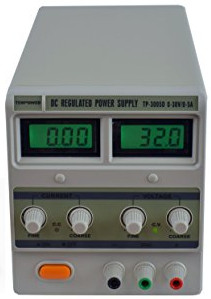
\includegraphics[scale=1.7]{lab_psu_cropped.jpg} 
\hspace{5mm} 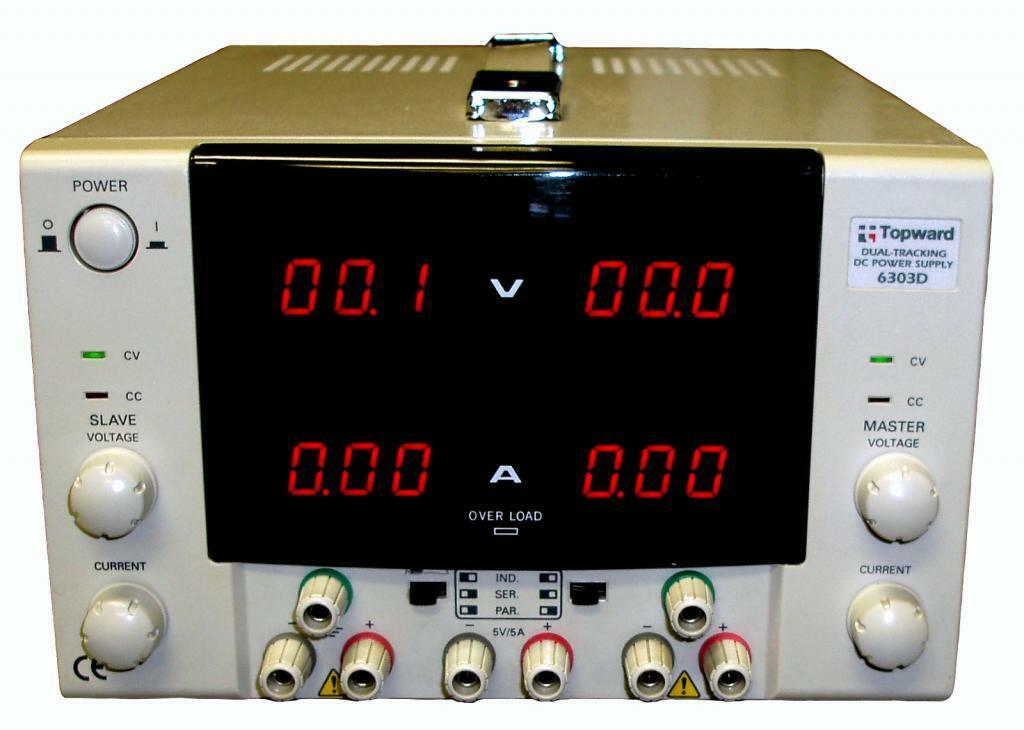
\includegraphics[scale=.17]{topward.jpg}
 
}

% Section II - Frame II:
\frame{  \small
\frametitle{\sectiontitleII}
 
 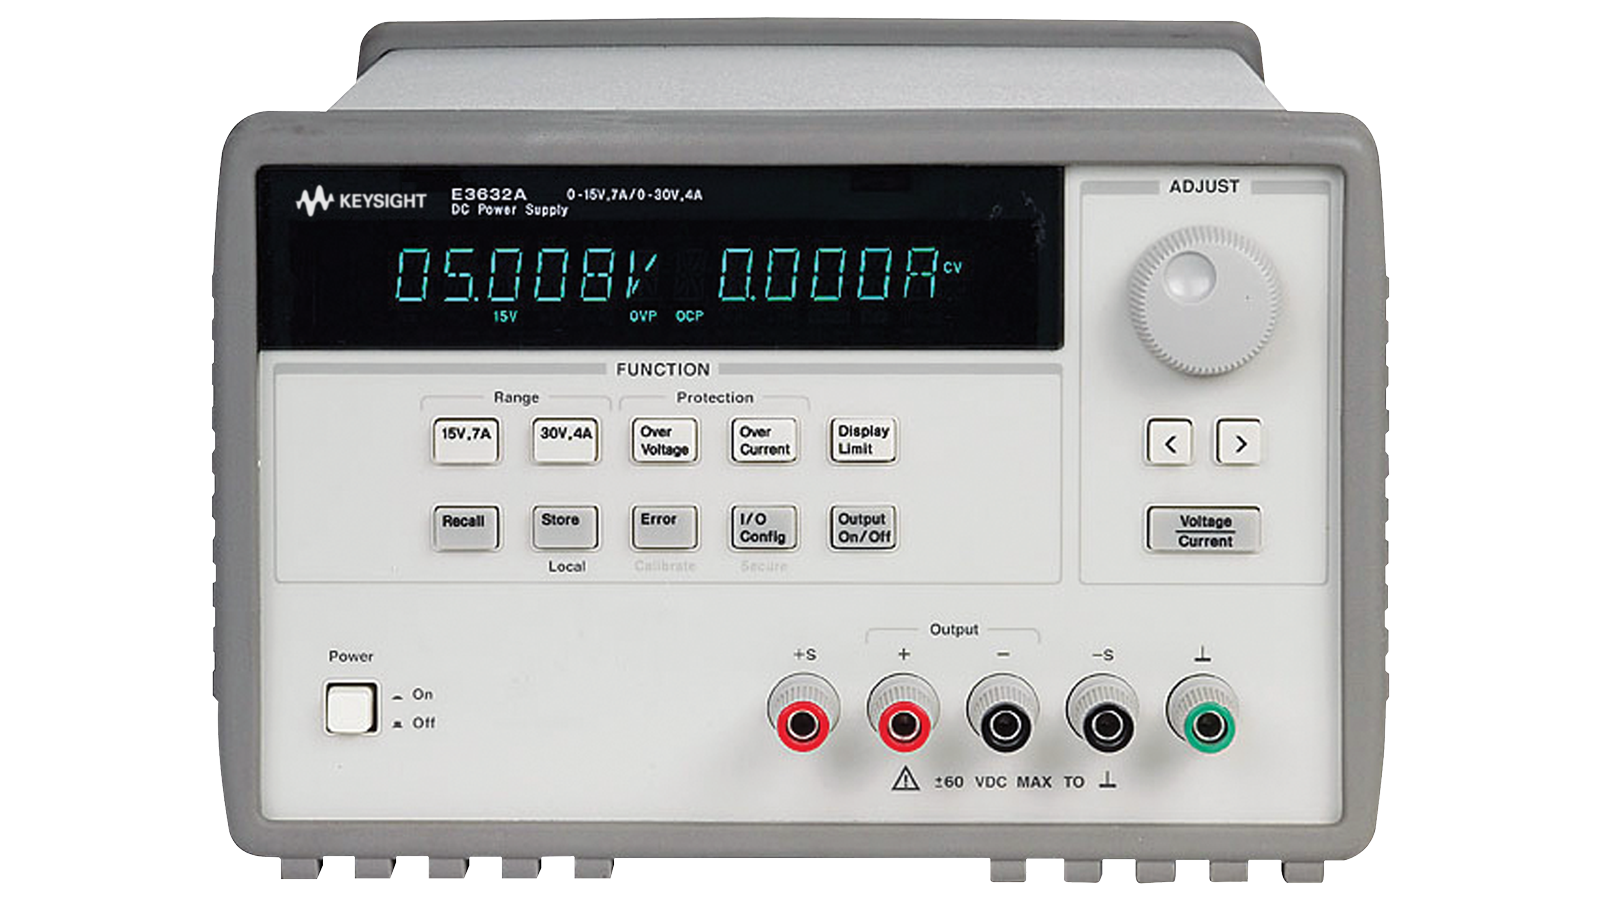
\includegraphics[scale=.15]{hp_psu.png} 

 
}


\section{\sectiontitleIII}

% Section II - Frame I:
\frame{  \small
\frametitle{\sectiontitleIII}
 
 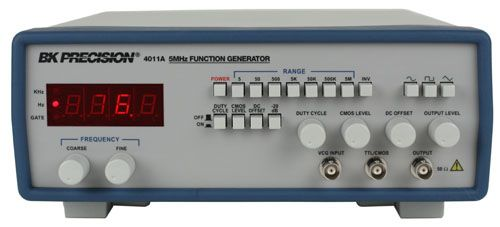
\includegraphics[scale=.5]{fn_gen.jpg}
 %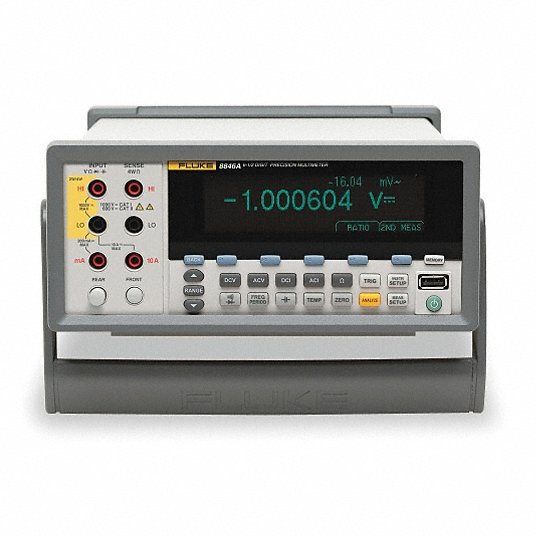
\includegraphics[scale=.30]{dmm_benchtop.jpeg}
 
}

% Section II - Frame I:
\frame{  \small
\frametitle{\sectiontitleIII}
 
 \underline{Thought Exercise:} How does a function generator work? \vspace{5mm}\\ \hspace{30mm} What is in the box?
 \vspace{40mm}
 
}

% Section III - Frame II:
\frame{  \small
\frametitle{\sectiontitleIII}



}

\section{\sectiontitleIV}

% Section IV - Frame I:
\frame{  \small
\frametitle{\sectiontitleIV}

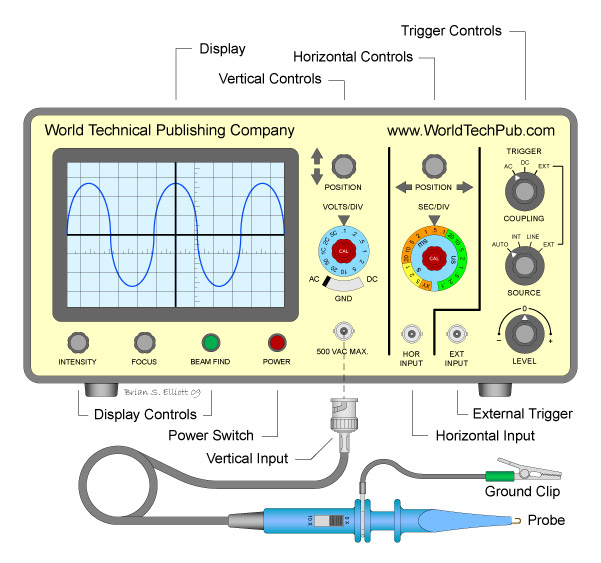
\includegraphics[scale=.5]{oscilloscope_fig1.jpg}



}

% Section IV - Frame II:
\frame{  \small
\frametitle{\sectiontitleIV}

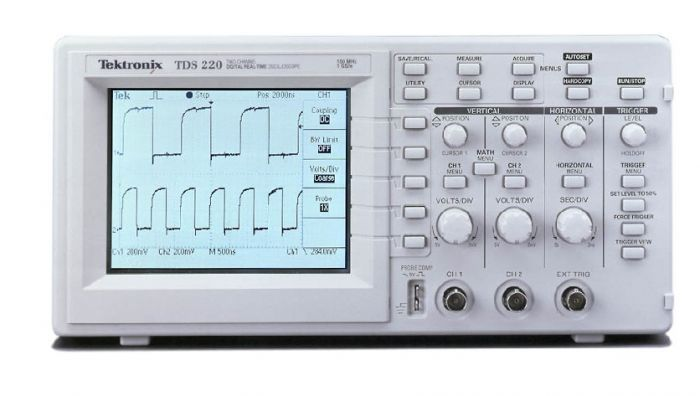
\includegraphics[scale=.35]{tds220.jpg}



}


\end{document}
%\begin{document}
%
%\textbf{ \LARGE ME3023 Lecture -  Chapter \NUM \\\\ \hspace*{5mm} Analog Electrical Devices
%and Measurements} \\\\
%\textbf{ \hspace*{5mm}\underline{Theory and Design for Mechanical Measurements}\vspace{1mm}\\ 
%                \hspace*{5mm} 5th ed. by Richard Figliola and Donald Beasley}\vspace{3mm}\\
%\textbf{ \hspace*{5mm}Tristan Hill - Tennessee Technological University - Fall 2019} \vspace{3mm}\\
%
%\begin{itemize}
%
%
%	\item \textbf{ \LARGE 6.1 -  Introduction  } \\\\
%	
%		\textbf{\Large "... basic electrical analog devices used with analog signals or to display signals in an analog form ..."} \\\\
%		 
%		\textbf{\Large " ... Information is often transferred between stages of a
%measurement system as an analog electrical signal. This signal typically originates from the
%measurement of a physical variable using a fundamental electromagnetic or electrical phenomenon
%and then propagates from stage to stage of the measurement system ... "} \\\\
%		\textbf{\Large "...  Within a signal chain, it is common to find digital and analog electrical devices being used together ...} \\
%
%\newpage		
%		 \textbf{\Large Upon completion of this chapter, the reader will be able to}\\\\
%		
%		\begin{itemize}
%			\item \textbf{\Large understand the principles behind common analog voltage and current measuring
%devices} \vspace{10mm}
%			\item \textbf{\Large understand the operation of balanced and unbalanced resistance bridge circuits} \vspace{10mm}
%			\item \textbf{\Large define, identify, and minimize loading errors}  \vspace{10mm}
%\item \textbf{\Large  understand the basic principles involved in signal conditioning, especially filtering and
%amplification, and }  \vspace{10mm}
%\item \textbf{\Large  apply proper grounding and shielding techniques in measuring system hookups.}  \vspace{10mm}
%		\end{itemize}
%		
%		\newpage
%	
%	\item \textbf{ \LARGE 6.1.0 -  BASIC ANALOG COMPONENTS : } \\
%\newpage
%	\item \textbf{ \LARGE 6.1.1 -  IMPORTANT QUANTITIES : } \\
%\newpage
%\item \textbf{ \LARGE 6.1.2 -  GOVERNING MATHEMATICS : } \\
%\newpage
%	\item \textbf{ \LARGE 6.1.3 -  PERFORMING ANALOG MEASUREMENTS: } \\
%\begin{itemize}
%
%		\item \textbf{ \LARGE \href{https://www.fluke.com/en-us/learn/best-practices/test-tools-basics/digital-multimeters/how-to-measure-resistance}{Measuring Resistance} } \vspace{130mm}\\ 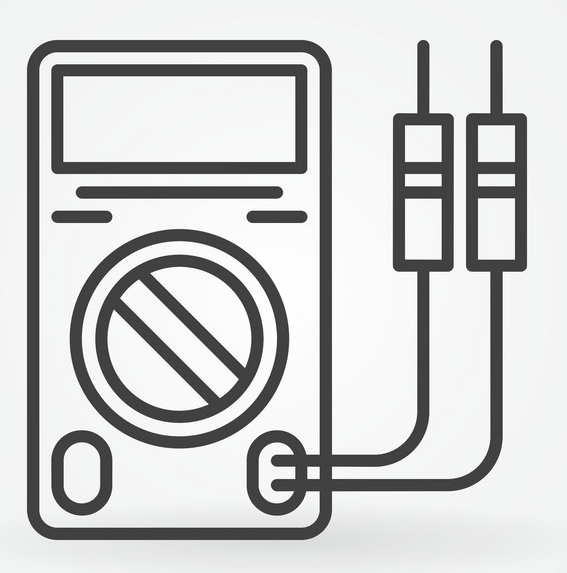
\includegraphics[scale=0.25]{lecture1_fig10.png} \\
%\newpage
%		\item \textbf{ \LARGE \href{https://www.fluke.com/en-us/learn/best-practices/test-tools-basics/digital-multimeters/how-to-test-for-continuity-with-a-digital-multimeter}{Continuity} } \vspace{130mm}\\ 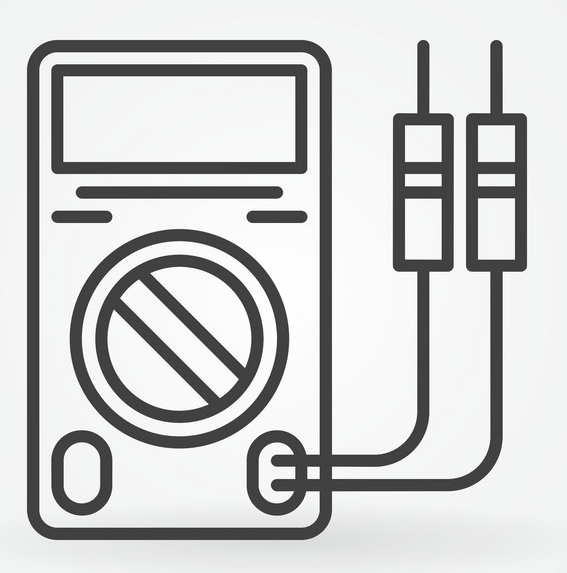
\includegraphics[scale=0.25]{lecture1_fig10.png} \\
%\newpage
%\item \textbf{ \LARGE \href{https://www.fluke.com/en-us/learn/best-practices/test-tools-basics/digital-multimeters/how-to-measure-capacitance-with-a-digital-multimeter}{Capacitance} } \vspace{130mm}\\ 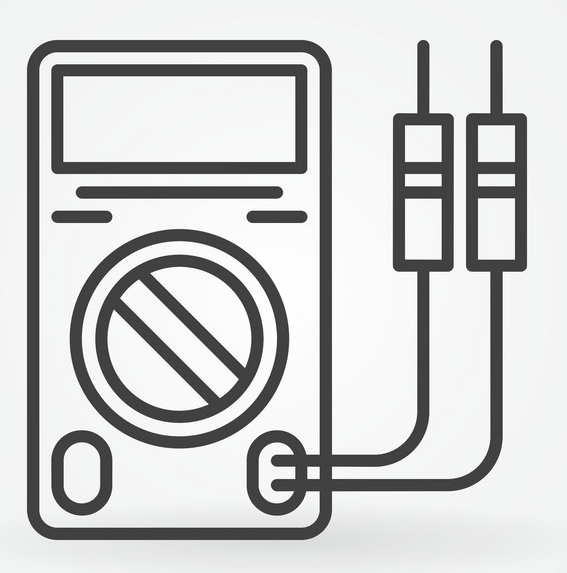
\includegraphics[scale=0.25]{lecture1_fig10.png} \\
%\newpage
%\item \textbf{ \LARGE \href{https://www.fluke.com/en-us/learn/best-practices/test-tools-basics/digital-multimeters/how-to-measure-dc-voltage-with-a-digital-multimeter}{DC voltage} }\vspace{130mm}\\ 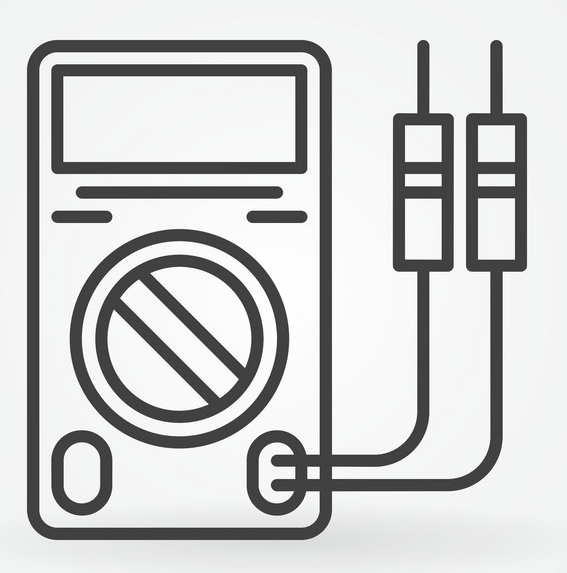
\includegraphics[scale=0.25]{lecture1_fig10.png} \\
%\newpage
%\item \textbf{ \LARGE \href{https://www.fluke.com/en-us/learn/best-practices/test-tools-basics/digital-multimeters/how-to-measure-ac-voltage-with-a-digital-multimeter}{AC voltage} }\vspace{130mm}\\ 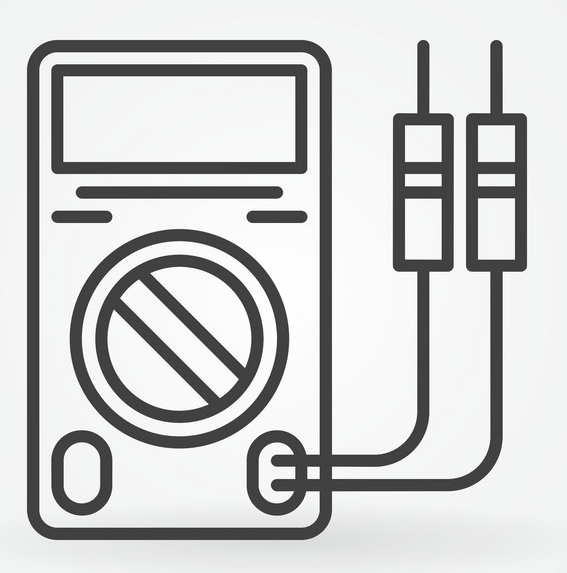
\includegraphics[scale=0.25]{lecture1_fig10.png} \\
%\newpage
%\item \textbf{ \LARGE \href{https://www.fluke.com/en-us/learn/best-practices/test-tools-basics/digital-multimeters/how-to-measure-current-with-a-digital-multimeter-plus-clamp-accessory}{Current (with clamp)} }\vspace{130mm}\\ 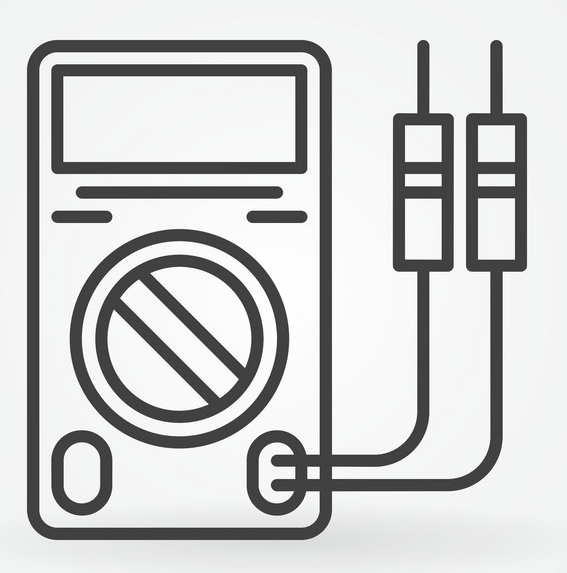
\includegraphics[scale=0.25]{lecture1_fig10.png} \\
%
%\end{itemize}
%
%	\newpage
%	\item \textbf{ \LARGE 6.2 -  ANALOG DEVICES: CURRENT } \\\\
%	\begin{itemize}
%		\item \textbf{ \LARGE Direct Current  } \\\\
%
%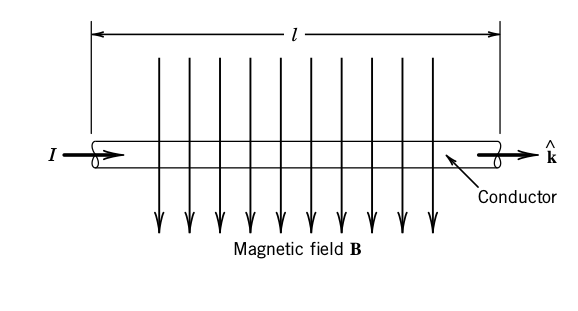
\includegraphics[scale=0.5]{lecture1_fig6_1.png} \\
%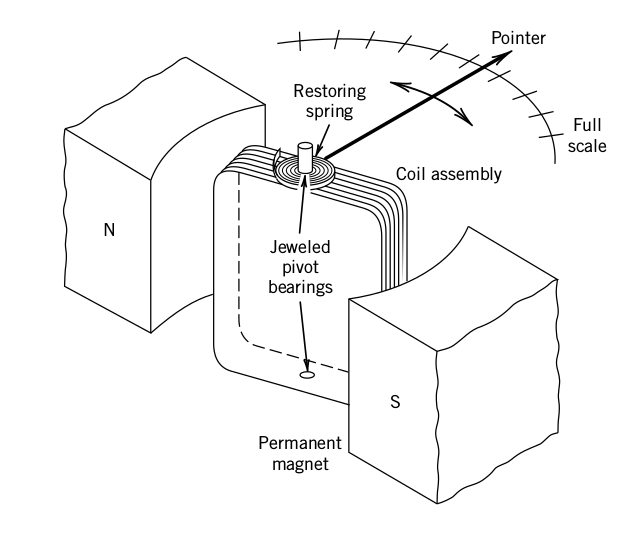
\includegraphics[scale=0.5]{lecture1_fig6_3.png}
%
%\scalebox{1}{$F=IlB$} \\
%\scalebox{1}{$\bf{F}=Il\hat{\bf{k}}\times\bf{B}$} \\
%\scalebox{1}{$T_{mu}=NIABsin{\alpha}$} \\
%
%\newpage
%		\item \textbf{ \LARGE Alternating Current} \\\\
%
%	\end{itemize}
%
%	\newpage
%	\item \textbf{ \LARGE 6.3 - ANALOG DEVICES: VOLTAGE} \\
%	\begin{itemize}
%		\item \textbf{ \LARGE Analog Voltage Meters  } \\
%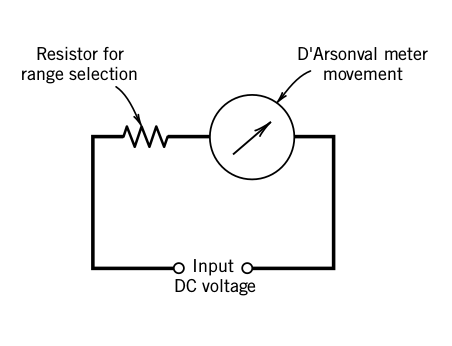
\includegraphics[scale=0.75]{lecture1_fig6_6.png} \\
%		\item \textbf{ \LARGE Oscilloscope} \\
%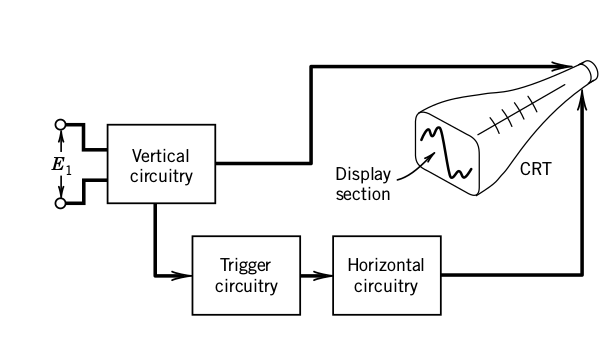
\includegraphics[scale=0.75]{lecture1_fig6_7.png} \\
%		\item \textbf{ \LARGE Potentiometer} \\\\
%		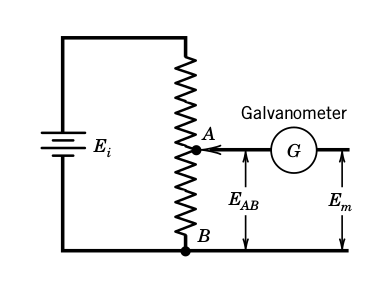
\includegraphics[scale=0.75]{lecture1_fig6_10.png} \\
%		\begin{itemize}
%			\item \textbf{ \LARGE Voltage Divider Circuit} \\\\
%
%
%
%			\item \textbf{ \LARGE Potentiometer Instruments} \\\\
%	
%		\end{itemize}
%	\end{itemize}
%
%	\newpage
%	\item \textbf{ \LARGE 6.4 -  ANALOG DEVICES: Resistance } \\\\
%	\begin{itemize}
%		\item \textbf{ \LARGE Ohmmeter Circuits  } \\\\
%		\item \textbf{ \LARGE Bridge Circuits} \\\\
%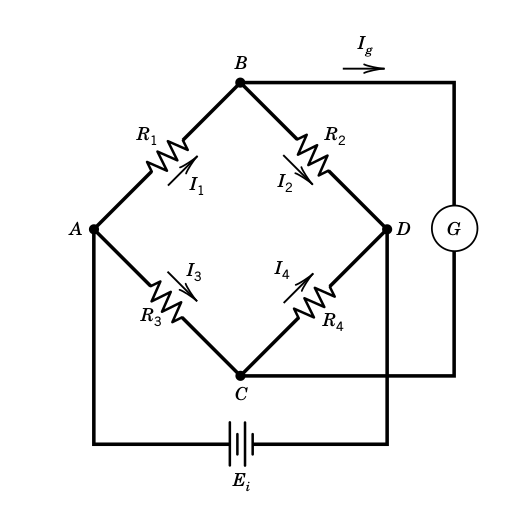
\includegraphics[scale=0.75]{lecture1_fig6_13.png} \\
%
%\newpage
%		\item \textbf{ \LARGE Null Method} \\\\
%		\item \textbf{ \LARGE Deflection Method} \\\\
%
%	\end{itemize}
%	
%\newpage
%	\item \textbf{ \LARGE 6.5 -  LOADING ERRORS AND IMPEDANCE MATCHING } \\\\
%	\begin{itemize}
%		\item \textbf{ \LARGE Loading Errors for Voltage-Dividing Circuit  } \\\\
%		\item \textbf{ \LARGE Interstage Loading Errors} \\\\
%
%	\end{itemize}
%
%\newpage
%	\item \textbf{ \LARGE 6.6 -  ANALOG SIGNAL CONDITIONING: AMPLIFIERS } \\\\
%	\begin{itemize}
%		\item \textbf{ \LARGE Operational Amplifiers} \\\\
%		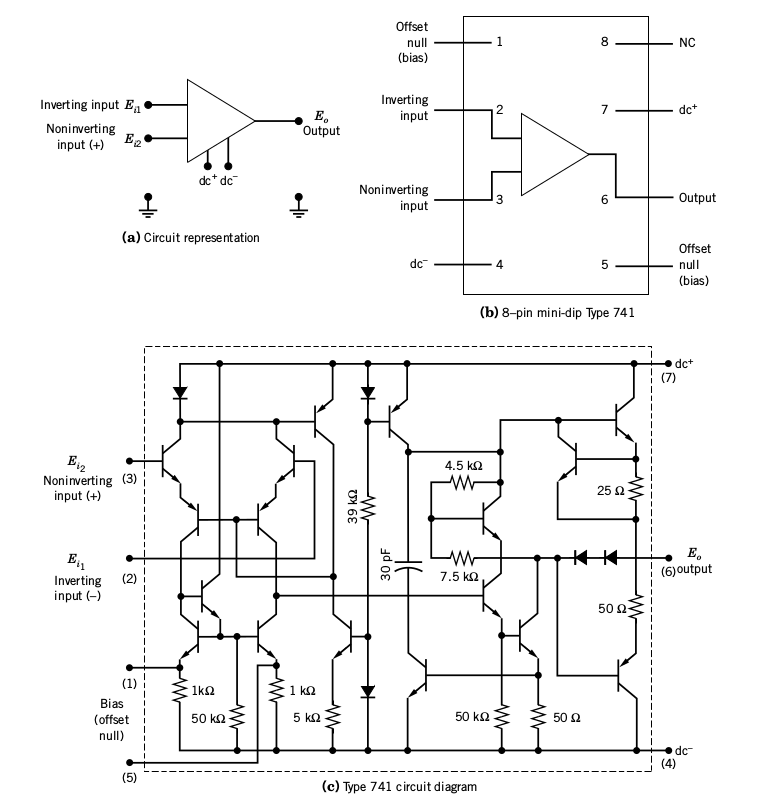
\includegraphics[scale=0.6]{lecture1_fig6_19.png} \\\\
%
%\item \textbf{ \LARGE Operational Amplifiers} \\\\
%		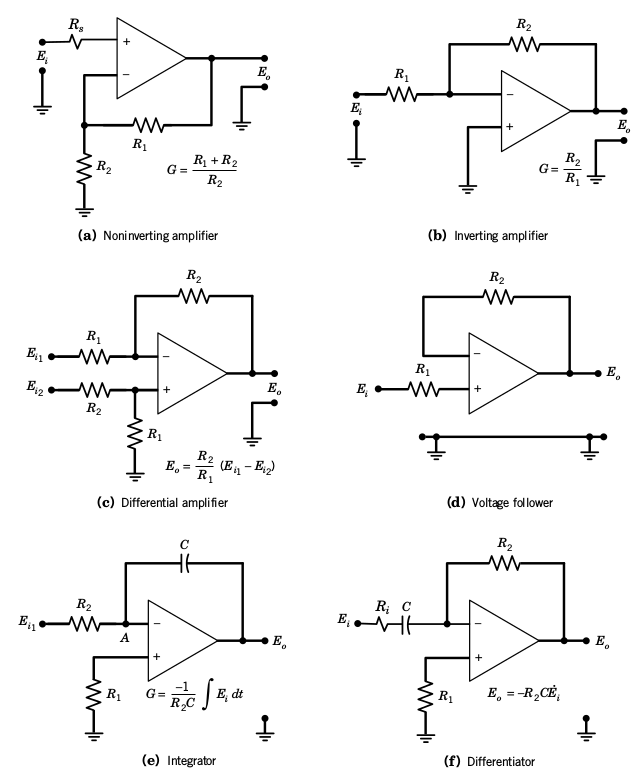
\includegraphics[scale=0.6]{lecture1_fig6_20.png} \\
%	\end{itemize}	
%\newpage
%
%	\item \textbf{ \LARGE 6.7 -  ANALOG SIGNAL CONDITIONING: SPECIAL-PURPOSE CIRCUITS } \\\\
%	\begin{itemize}
%		\item \textbf{ \LARGE Analog Voltage Comparator} \\\\
%		\item \textbf{ \LARGE Sample-and-Hold Circuit} \\\\
%		\item \textbf{ \LARGE Charge Amplifier} \\\\
%		\item \textbf{ \LARGE 4-20mA Current Loop} \\\\
%		\item \textbf{ \LARGE Multivibrator and Flip-Flop Circuits} \\\\
%	\end{itemize}	
%\newpage
%	\item \textbf{ \LARGE 6.8 -  ANALOG SIGNAL CONDITIONING: Filters } \\\\
%
%		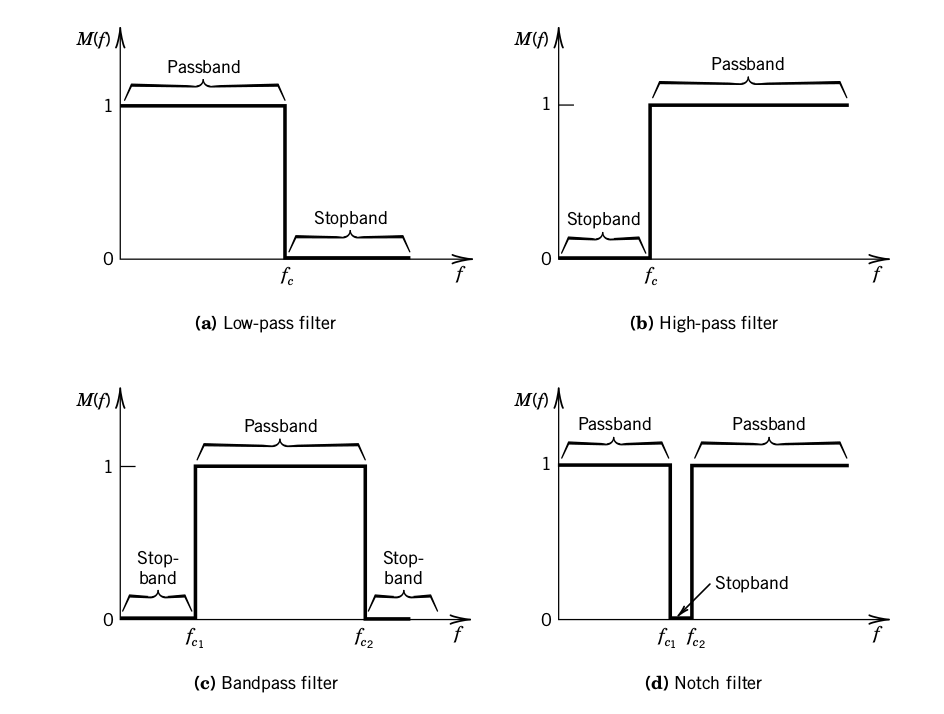
\includegraphics[scale=0.45,angle=0,origin=c]{lecture1_fig6_27.png} \\
%		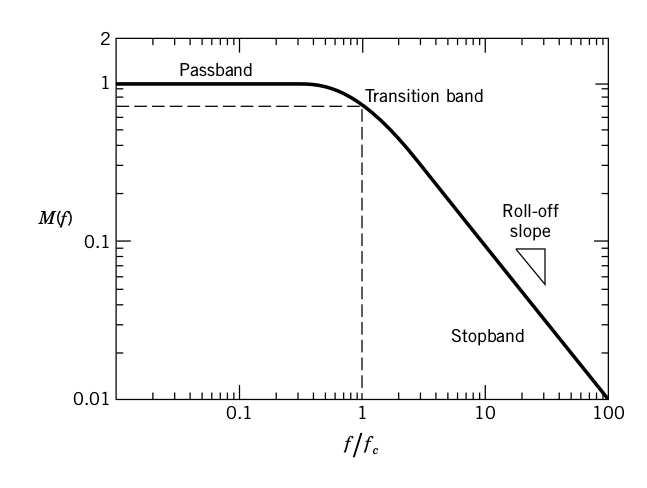
\includegraphics[scale=0.45]{lecture1_fig6_28.png} \\
%	\begin{itemize}
%		\item \textbf{ \LARGE Butterworth Filter Design} \\\\
%		\item \textbf{ \LARGE Improved Butterworth Filter Designs} \\\\
%		\item \textbf{ \LARGE Bessel Filter Design} \\\\
%		\item \textbf{ \LARGE Active Filters} \\\\
%	\end{itemize}	
%\newpage
%	\item \textbf{ \LARGE 6.9 GROUNDS, SHIELDING, AND CONNECTING WIRES } \\\\
%	\begin{itemize}
%		\item \textbf{ \LARGE Ground and Ground Loops} \\\\
%		\item \textbf{ \LARGE Connecting Wires} \\\\
%	\end{itemize}	
%\newpage
%	\item \textbf{ \LARGE 6.10 SUMMARY } \\\\
%	\begin{itemize}
%		\item \textbf{ \LARGE woop woop} \\\\
%	\end{itemize}	
%
%		%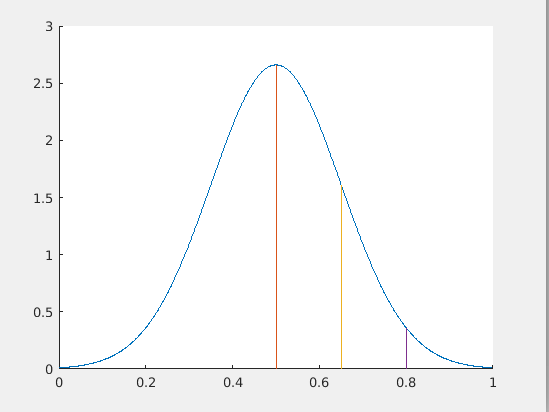
\includegraphics[scale=1]{lecture1_fig1.png}
%		
%\end{itemize}
%
%
%	
%
%\end{document}
%
%
%
